\section{Problemstellung und grafische Lösung}

\stepcounter{subsection}% Nummerierung 2.1.1.x

Gegenstand der \textbf{Linearen Optimierung} ist es, aus derartigen Lösungsmengen besondere Lösungen herauszusuchen, die hinsichtlich eines zusätzlich gegebenen Kriteriums optimal sind. Es wird nun mit einem konkreten Beispiel fortgefahren, aus dem sich eine solche Fragestellung in typischer Weise ergibt.

\subsubsection{Übungsaufgabe}

\begin{graukasten}
  Stellen Sie das Lösungsgebiet des folgenden Systems von Ungleichungen grafisch dar:
  \[ 3x_1 + 2x_2 \leq 24, \quad x_2 \leq 8, \quad x_1, x_2 \geq 0 . \]
\end{graukasten}

\subsubsection{Beispiel}

Ein Unternehmen stellt die beiden Produkte $P_1$ und $P_2$ auf den drei Maschinen $M_1$, $M_2$ und $M_3$ her. Im Laufe eines Jahres steht Maschine $M_1$ höchstens 3000 Stunden, $M_2$ höchstens 750 Stunden und $M_3$ höchstens 1200 Stunden zur Verfügung. Für eine Einheit von Produkt $P_1$ verlangt auf Maschine $M_1$ eine Bearbeitungszeit von 5 Stunden, zusätzlich benötigt man auf $M_3$ 4 Stunden; $M_2$ wird zur Herstellung von $P_1$ nicht benötigt. Für eine Einheit von Produkt $P_2$ lauten die entsprechenden Bearbeitungszeiten 10 Stunden auf Maschine $M_1$, 3 Stunden auf $M_2$ und 2 Stunden auf $M_3$. Jede Maschine kann zu einem Zeitpunkt nur für eines der beiden Produkte verwendet werden; für ein Produkt ist es unerheblich, in welcher Reihenfolge es auf den einzelnen Maschinen bearbeitet wird. Der Stückgewinn für Produkt $P_1$ beträgt 200 Euro, für $P_2$ 300 Euro.

Wieviele Einheiten der beiden Produkte sollte das Unternehmen in einem Jahr herstellen, um seinen Gewinn zu maximieren?\beispielende

Um zu verdeutlichen, dass in dem Beispiel eine echte Problemstellung vorliegt, deren Lösung nicht völlig simpel ist, sei auf folgendes hingewiesen: Beispielsweise könnten 250 Einheiten von Produkt $P_2$ und \emph{keine} von Produkt $P_1$ hergestellt werden. In diesem Falle wäre Maschine $M_2$ (mit 750 Betriebsstunden) voll ausgelastet, $M_1$ und $M_3$ hätten noch Kapazitäten frei. Der Gewinn würde dann $250 \cdot 300$ Euro bzw. 75000 Euro betragen.

Eine andere Möglichkeit wäre es, je 200 Einheiten von $P_1$ und $P_2$ zu produzieren. In diesem Fall wären $M_1$ und $M_3$ voll ausgelastet, der Gewinn beträgt $200 \cdot 200 + 200 \cdot 300$ Euro bzw. 100000 Euro.

Die zweite Möglichkeit führt also zu einem höheren Gewinn. Gibt es eine noch bessere Lösung?

Probleme dieser Art tauchen in den Wirtschaftswissenschaften sehr häufig auf. Da das Wort »höchstens« in der Problemstellung eine zentrale Rolle spielt, liegt es auf der Hand, dass die mathematische Formulierung des Problems zu \emph{Ungleichungen} führt -- dies wird nun genauer dargestellt, und zwar anhand des gewählten Beispiels.

\subsubsection{Fortsetzung des Beispiels}

Für die unbekannten Mengen der herzustellenden Produkte $P_1$ und $P_2$ werden zunächst die Variablen $x_1$ und $x_2$ eingeführt, die als \textbf{Entscheidungsvariablen} bezeichnet werden. Durch die zeitliche Nutzbarkeit der drei Maschinen ergeben sich nun die folgenden Ungleichungen, die den Variablen \textbf{Restriktionen} auferlegen:
\begin{align*}
  5x_1 + 10x_2 &\leq 3000 \qquad (\text{Maschine 1})\\
  3x_2 &\leq 750 \qquad (\text{Maschine 2})\\
  4x_1 + 2x_2 &\leq 1200 \qquad (\text{Maschine 3})
\end{align*}
Man spricht hier auch von den \textbf{einschränkenden Bedingungen}. Der Vollständigkeit halber kommen noch die \textbf{Nichtnegativitätsbedingungen}
\[ x_1 \geq 0, \; x_2 \geq 0 \]
hinzu, denn »negative Stückzahlen« brauchen nicht betrachtet zu werden. Dadurch wird das mathematische Problem nochmals stark eingeschränkt.

Bisher ist zwar von zahlreichen \textbf{Bedingungen} die Rede gewesen, jedoch gibt es immer noch mehrere Kombinationen von $x_1$- und $x_2$-Werten, die alle diese Bedingungen erfüllen. Es ist aber zusätzlich die sogenannte \textbf{Zielfunktion}
\[ Z = 200 x_1 + 300 x_2 \]
zu beachten, die in unserem Beispiel den Gewinn darstellt und die es zu maximieren gilt.

Die durch das gewählte Beispiel gegebene Problemstellung ist nun vollständig durch ein mathematisches Modell erfasst. In Kurzform stellt man dieses Modell üblicherweise in der folgenden Form dar:
\begin{center}
  \fbox{\begin{minipage}{0.8\linewidth}
    \begin{align*}
      Z &= 200 x_1 + 300 x_2 \rightarrow Max!\\
      5x_1 + 10x_2 &\leq 3000\\
      3x_2 &\leq 750\\
      4x_1 + 2x_2 &\leq 1200\\
      x_j &\geq 0 \quad (j = 1,2)
    \end{align*}
  \end{minipage}}
\end{center}

Die Lösung des Problems soll nun auf grafische Weise gefunden werden. Wenn konkrete Werte für $x_1$ und $x_2$ sämtliche der obigen Ungleichungen erfüllen, so spricht man von \textbf{zulässigen Werten}; alle zulässigen Wertepaare bilden den \textbf{zulässigen Bereich}. Ein zulässiges Wertepaar mit maximalem $Z$-Wert ist \textbf{optimal}; es kann dabei durchaus mehrere optimale Wertepaare geben (dann natürlich mit dem gleichen maximalen $Z$-Wert).

Für das Beispiel ist hier im Bild der zulässige Bereich dargestellt:

\begin{center}
  \begin{tikzpicture}
    \begin{axis}[width=10cm, height=7.5cm, axis lines=left, xmin=0, xmax=400, ymin=0, ymax=400,
      xtick={100,200,300}, ytick={100,200,300}, xlabel={$x_1$}, ylabel={$x_2$}, tick label style={font=\footnotesize}, samples=50,
      clip=true]
      \addplot[black, thick, domain=0:300] {600-2*x};
      \addplot[black, thick, domain=0:400] {250};
      \addplot[black, thick, domain=0:400] {300-0.5*x};
      \fill[gray!30] (axis cs:0,0) -- (axis cs:0,250) -- (axis cs:100,250) -- (axis cs:200,200) -- (axis cs:300,0) -- cycle;
      \node[above right] at (axis cs:200,320) {$x_2 = 600 - 2x_1$};
      \node[above] at (axis cs:350,255) {$x_2 = 250$};
      \node[below right] at (axis cs:330,70) {$x_2 = 300 - \tfrac{1}{2}x_1$};
    \end{axis}
  \end{tikzpicture}
\end{center}

Der schraffierte Bereich besteht aus allen Punkten, die
\begin{itemize}
  \item unterhalb der Geraden $x_2 = 300 - \tfrac{1}{2}x_1$,
  \item unterhalb der Geraden $x_2 = 250$,
  \item unterhalb der Geraden $x_2 = 600 - 2x_1$,
  \item im ersten Quadranten
\end{itemize}
liegen.

Gesucht ist mit anderen Worten ein Punkt $(x_1, x_2)$ des schraffierten Bereichs, für den
\[ Z = 200 x_1 + 300 x_2 \]
möglichst groß ist. Um sich diesem Problem zu nähern, setze man einmal für $Z$ einen konkreten Wert ein, etwa 60000:
\[ 60000 = 200 x_1 + 300 x_2 \]
bzw.
\[ x_2 = 200 - \tfrac{2}{3} x_1 \]
ist wieder eine Geradengleichung. Die Gerade wird in das Bild eingezeichnet, wobei man sie der Einfachheit halber mit »$Z = 60000$« beschriftet.

Das Geradenstück, welches innerhalb des schraffierten Bereiches verläuft, stellt nun offensichtlich alle diejenigen zulässigen Punkte $(x_1; x_2)$ dar, die jeweils zu einem Gewinn von genau 60000 Euro führen. Man spricht von einer \textbf{Isogewinngeraden}. Um klarzumachen, worauf die Argumentation hinausläuft, werden nun zwei weitere $Z$-Werte gewählt, nämlich $Z = 100000$ und $Z = 110000$. Die zugehörigen Geraden sind in folgendem Bild eingezeichnet.

Wie man sieht, ergeben die unterschiedlichen $Z$-Werte parallele Geraden. Für $Z = 100000$ enthält die Gerade nur noch einen zulässigen Punkt, nämlich $x_1 = 200$ und $x_2 = 200$. Für $Z = 110000$ hat die zugehörige Gerade keinen Punkt mehr mit dem schraffierten Bereich gemeinsam -- mithin existiert keine zulässige Lösung, die einen Gewinn von 110000 Euro liefert.

\fbox{\begin{minipage}{0.9\linewidth}
  Folglich ist der Punkt $(x_1; x_2) = (200;200)$ die Lösung des Problems, der maximale Gewinn beträgt $Z = 100000$ Euro.
\end{minipage}}\beispielende

Löst man sich nun gedanklich von dem konkreten Beispiel, so legt die soeben vollzogene grafische Lösungsmethode doch allgemein nahe, dass das Optimum immer in einem \textbf{Eckpunkt} des zugrundeliegenden zulässigen Bereiches angenommen wird. Bereiche der dargestellten Art mit endlichem Flächeninhalt, die sich als Überschneidungsbereich mehrerer Halbebenen ergeben, heißen allgemein \textbf{Polyeder}, in dem hier vorliegenden Zusammenhang \textbf{Lösungspolyeder}. Dass das Interesse auf dessen Eckpunkte zu richten ist, soll hier nicht formal mathematisch bewiesen werden. Die Grundidee des Simplex-Algorithmus, der im nächsten Abschnitt vorgestellt wird, besteht darin, von Ecke zu Ecke zu »laufen« und auf diese Weise eine optimale Lösung zu finden.

\subsubsection{Übungsaufgabe}

\begin{graukasten}
  Gegeben ist folgendes Standard-Maximum-Problem: $Z = 4x_1 + x_2 \rightarrow Max$. Die Nebenbedingungen sind:
  \[ 3x_1 + 2x_2 \leq 24, \quad x_2 \leq 8, \quad x_1, x_2 \geq 0 . \]
  Ermitteln Sie grafisch das Maximum. Wie groß ist der maximale $Z$-Wert?
\end{graukasten}

\section{Der Simplex-Algorithmus}

\stepcounter{subsection}% Nummerierung 2.2.1.x

In diesem Abschnitt wird ein allgemeines Verfahren vorgestellt, mit dessen Hilfe man Probleme der vorgestellten Art lösen kann. Bei einem solchen \textbf{linearen Optimierungsproblem mit $n$ Entscheidungsvariablen}, in dem die (ebenfalls lineare) Zielfunktion \textbf{maximiert} werden soll, spricht man von einem \textbf{Standard-Maximum-Problem}.

Die folgende Situation liegt also vor:
\begin{enumerate}[label=\Roman*)]
  \item Man hat \textbf{Entscheidungsvariablen} $x_1, x_2, \ldots, x_i, \ldots, x_n$ $(n \geq 2)$.
  \item Es ist eine \textbf{lineare Zielfunktion}
    \[ Z = c_1 x_1 + c_2 x_2 + \ldots + c_i x_i + \ldots + c_n x_n \rightarrow Max! \]
    gegeben, deren Wert durch geeignete Wahl der $x_i$ maximiert werden soll.
  \item Es gelten \textbf{lineare Restriktionen}:
    \begin{align*}
      a_{11} x_1 + a_{12} x_2 + \ldots + a_{1n} x_n &\leq b_1\\
      &\vdots\\
      a_{m1} x_1 + a_{m2} x_2 + \ldots + a_{mn} x_n &\leq b_m\\
      & (b_i \geq 0 \text{ für alle } i = 1,2,\ldots,m)
    \end{align*}
  \item Es gelten die \textbf{Nichtnegativitätsbedingungen} $x_1, x_2, \ldots, x_n \geq 0$.
\end{enumerate}

In dem im vorigen Abschnitt behandelten Beispiel ist $n = 2$ und $m = 3$. Dabei konnte die optimale Lösung auf grafische Weise ermittelt werden. Sind mehr als zwei Entscheidungsvariablen im Spiel, ist das zeichnerische Verfahren jedoch nicht geeignet.

Der \textbf{Simplex-Algorithmus} geht von einem solchen Standard-Maximum-Problem aus. Wie dieses Verfahren abzuwandeln ist, wenn ein lineares Optimierungsproblem in anderer Form vorliegt, wird im nächsten Abschnitt angesprochen. (Beispielsweise könnte es alternativ das Ziel sein, die Zielfunktion zu \emph{minimieren}, oder einige lineare Restriktionen könnten als $\geq$-Beziehungen gegeben sein.) Der Algorithmus arbeitet, wie bald gezeigt wird, mit einer Darstellung des Problems in Form rechteckiger Zahlenschemata, sogenannter \textbf{Tableaus}. Dies ähnelt der Matrizendarstellung, die bei der Behandlung linearer Gleichungssysteme verwendet wurde. Auch der Simplex-Algorithmus selbst weist in seinen typischen Operationen Ähnlichkeiten zum Gaußschen Algorithmus zur Lösung linearer Gleichungssysteme auf.

Der Simplex-Algorithmus wird nun anhand des im vorigen Abschnitt eingeführten Beispiels erläutert. Anschließend wird ein weiteres Beispiel (mit drei Entscheidungsvariablen) durchgerechnet, um die Vorgehensweise nochmals zu illustrieren. Auf eine vollständige formale Beschreibung des Algorithmus (mit beliebiger Anzahl $n$ von Entscheidungsvariablen) wird verzichtet.

Ausgegangen wird von dem mathematischen Modell, das für das Beispielproblem im vorigen Abschnitt aufgestellt wurde:
\begin{center}
  \fbox{\begin{minipage}{0.8\linewidth}
    \begin{align*}
      Z &= 200 x_1 + 300 x_2 \rightarrow Max!\\
      5x_1 + 10x_2 &\leq 3000\\
      3x_2 &\leq 750\\
      4x_1 + 2x_2 &\leq 1200\\
      x_j &\geq 0 \quad (j = 1,2)
    \end{align*}
  \end{minipage}}
\end{center}

Das Ungleichungssystem der linearen Restriktionen wird nun durch Hinzufügen von sogenannten \textbf{Schlupfvariablen} $y_1$, $y_2$ und $y_3$ in ein Gleichungssystem überführt:
\begin{align*}
  5x_1 + 10x_2 + y_1 &= 3000\\
  3x_2 + y_2 &= 750\\
  4x_1 + 2x_2 + y_3 &= 1200
\end{align*}
Die Schlupfvariablen lassen sich für das Beispiel als die Leerlaufzeiten der Maschinen $M_1$, $M_2$ und $M_3$ deuten. (Bei anderen Problemstellungen trifft unter Umständen eine andere Interpretation zu.) Für die Schlupfvariablen muss ebenfalls die Nichtnegativitätsbedingung gelten:
\[ y_i \geq 0 \quad \text{für } i = 1,2,3 \]
Die Zielfunktion wird nun ebenfalls als Gleichung hingeschrieben:
\[ -200 x_1 - 300 x_2 + Z = 0 \]
Insgesamt ist auf diese Weise ein alternatives mathematisches Modell entstanden, welches aus vier Gleichungen mit sechs Variablen besteht:

\begin{center}
  \begin{tabular}{|rr|rrr|r|r|}
    \hline
    $5x_1$ & $+10x_2$ & $+y_1$ & & & & $= 3000$\\
    & $3x_2$ & & $+y_2$ & & & $= 750$\\
    $4x_1$ & $+2x_2$ & & & $+y_3$ & & $= 1200$\\
    $-200x_1$ & $-300x_2$ & & & & $+Z$ & $= 0$\\
    \hline
  \end{tabular}
\end{center}

Das sogenannte \textbf{Ausgangstableau} für den Simplex-Algorithmus wird nun erstellt, indem in der Kopfzeile die Namen der Variablen und darunter die Koeffizienten des Gleichungssystems eingetragen werden. Die Werte der jeweiligen rechten Seite werden mit $b_i$ gekennzeichnet. Für das Beispiel erhält man so zunächst:

\begin{center}
  \begin{tabular}{|r|r|r|r|r|r|r|}
    \hline
    $x_1$ & $x_2$ & $y_1$ & $y_2$ & $y_3$ & $Z$ & $b_i$\\
    \hline
    5 & 10 & 1 & 0 & 0 & 0 & 3000\\
    0 & 3 & 0 & 1 & 0 & 0 & 750\\
    4 & 2 & 0 & 0 & 1 & 0 & 1200\\
    -200 & -300 & 0 & 0 & 0 & 1 & 0\\
    \hline
  \end{tabular}
\end{center}

Wie man sieht, stehen in den Spalten, die zu den Schlupfvariablen gehören, jeweils \textbf{Basisvektoren}, die an einer Stelle eine 1 und sonst nur Nullen aufweisen (vgl. auch Kapitel 1). Im Verlauf des Algorithmus wird nun in jedem Schritt in einer anderen Spalte ein Basisvektor erzeugt, wobei die Variablen, in deren Spalten Basisvektoren stehen, \textbf{Basisvariablen} heißen; im obigen Tableau sind also die drei Schlupfvariablen und $Z$ die Basisvariablen.

Um stets erkennen zu können, welche Variablen gerade die Basisvariablen sind, fügt man üblicherweise eine zusätzliche erste Spalte hinzu, die mit »BV« (steht für: Basisvariablen) überschrieben ist und in die folglich zu Beginn die Schlupfvariablen und die zu maximierende Größe (also hier $y_1$, $y_2$, $y_3$ und $Z$) eingetragen werden:

\begin{center}
  \begin{tabular}{|r|r|r|r|r|r|r|r|}
    \hline
    BV & $x_1$ & $x_2$ & $y_1$ & $y_2$ & $y_3$ & $Z$ & $b_i$\\
    \hline
    $y_1$ & 5 & 10 & 1 & 0 & 0 & 0 & 3000\\
    $y_2$ & 0 & 3 & 0 & 1 & 0 & 0 & 750\\
    $y_3$ & 4 & 2 & 0 & 0 & 1 & 0 & 1200\\
    $Z$ & $-200$ & $-300$ & 0 & 0 & 0 & 1 & 0\\
    \hline
  \end{tabular}
\end{center}

Diese Darstellungsweise ähnelt derjenigen, die beim Gaußschen Algorithmus zur Lösung linearer Gleichungssysteme verwendet wurde. Entsprechend der jetzigen Intention, dieses Gleichungssystem nicht \emph{allgemein} zu lösen (d.\,h. \emph{alle} Lösungen zu finden), sondern vielmehr \emph{eine besondere} Lösung zu suchen, ist nun jedoch eine alternative Vorgehensweise angesagt. Wir werden aber sehen, dass dieselben Grundtechniken verwendet werden wie beim Gaußschen Algorithmus -- also Addition von Zeilen und Multiplikation von Zeilen mit irgendwelchen Zahlenwerten.

Zunächst stellt man fest, dass in dem Beispiel vier Gleichungen mit sechs Unbekannten vorliegen. Da die vier Zeilen des Tableaus offensichtlich linear unabhängig sind (also keine als Summe der anderen ausgedrückt werden kann), folgt daraus, dass zwei der sechs Variablen (beliebig) frei gewählt werden können -- die restlichen vier kann man dann berechnen. Die Grundidee des Simplex-Algorithmus besteht nun darin, zweien der Variablen $x_1$, $x_2$, $y_1$, $y_2$ oder $y_3$ den Wert Null zuzuweisen (die restlichen drei bilden dann mit $Z$ die Basisvariablen) und die zugehörige Lösung zu bestimmen; ist diese noch nicht optimal, so werden zwei andere Variablen auf Null gesetzt. Es stellt sich heraus, dass auf diese Weise die Ecken des Lösungspolyeders »durchlaufen« werden. Dies wird so lange durchgeführt, bis man auf eine optimale Lösung gestoßen ist.

Aufgrund dieser groben Skizze des Simplex-Algorithmus stellen sich sofort die folgenden Fragen:
\begin{itemize}
  \item Wieso \emph{muss} man bei dieser Vorgehensweise auf eine optimale Lösung stoßen?
  \item Woran sieht man, \emph{dass} man auf eine optimale Lösung gestoßen ist?
  \item Angenommen, man ist bei einer Lösung angelangt, die noch nicht optimal ist -- wie ist weiter vorzugehen, also welche Variablen setzt man als nächstes auf Null?
\end{itemize}
Alle diese Fragen werden bei der nun folgenden Beschreibung des Simplex-Algorithmus beantwortet.

Zunächst wird noch einmal auf die Abbildung geschaut, in der das Lösungspolyeder dargestellt ist. Das Polyeder wird durch die fünf Geraden
\[ x_2 = 300 - \tfrac{1}{2}x_1, \quad x_2 = 250, \quad x_2 = 600 - 2x_1, \quad x_2 = 0, \quad x_1 = 0 \]
eingegrenzt.

Im Allgemeinen können fünf Geraden bis zu 10 Schnittpunkte haben. Da hier aber die Geraden $x_2 = 250$ und $x_2 = 0$ parallel sind, ergeben sich nur neun Schnittpunkte. Diese sind in der folgenden Abbildung mit $E_0$, $E_1$, \ldots, $E_4$ (Ecken des Lösungspolyeders) und $E_5'$, \ldots, $E_8'$ (weitere Schnittpunkte) bezeichnet.

\begin{center}
  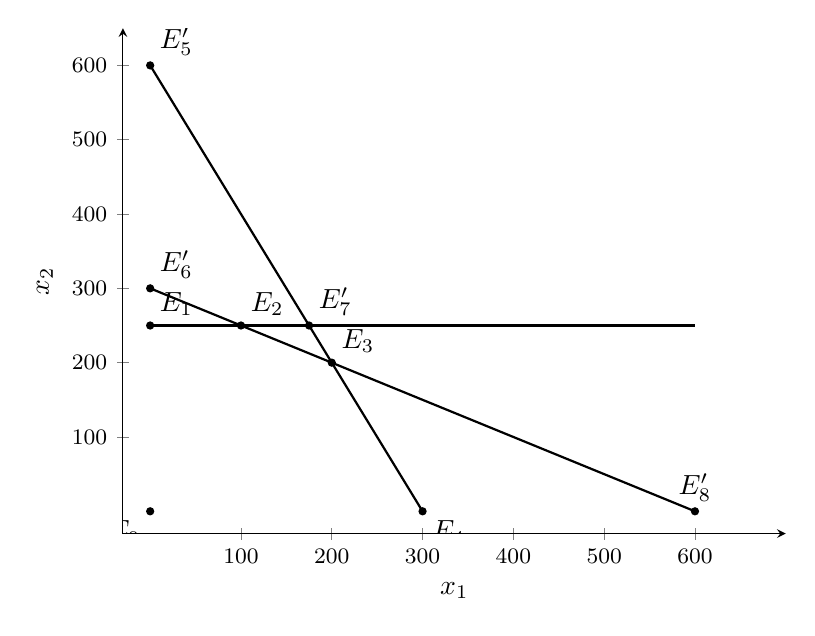
\begin{tikzpicture}
    \begin{axis}[width=10cm, height=8cm, axis lines=left, xmin=-30, xmax=700, ymin=-30, ymax=650,
      xtick={100,200,...,600}, ytick={100,200,...,600}, xlabel={$x_1$}, ylabel={$x_2$}, tick label style={font=\footnotesize}, samples=50,
      clip=true]
      \addplot[black, thick, domain=0:600] {300-0.5*x};
      \addplot[black, thick, domain=0:600] {250};
      \addplot[black, thick, domain=0:300] {600-2*x};
      \fill (axis cs:0,0) circle (1.5pt) node[below left] {$E_0$};
      \fill (axis cs:0,250) circle (1.5pt) node[above right] {$E_1$};
      \fill (axis cs:100,250) circle (1.5pt) node[above right] {$E_2$};
      \fill (axis cs:200,200) circle (1.5pt) node[above right] {$E_3$};
      \fill (axis cs:300,0) circle (1.5pt) node[below right] {$E_4$};
      \fill (axis cs:0,600) circle (1.5pt) node[above right] {$E_5'$};
      \fill (axis cs:0,300) circle (1.5pt) node[above right] {$E_6'$};
      \fill (axis cs:175,250) circle (1.5pt) node[above right] {$E_7'$};
      \fill (axis cs:600,0) circle (1.5pt) node[above] {$E_8'$};
    \end{axis}
  \end{tikzpicture}
\end{center}

Entscheidend ist nun die folgende Beobachtung:
\merkbox{Jeder Geradenschnittpunkt korrespondiert zu einer Auswahl von zwei der Variablen $x_1$, $x_2$, $y_1$, $y_2$, $y_3$, die den Wert Null annehmen.}

Die zwei Variablen, deren Wert Null ist, heißen -- wie bereits gesagt -- \textbf{Nichtbasisvariablen} ($NBV$), die anderen \textbf{Basisvariablen} ($BV$). Beispielsweise gilt in Punkt $E_0$: $x_1 = 0$ und $x_2 = 0$; im Punkt $E_5'$ sind $x_1 = 0$ und $y_3 = 0$. Von besonderem Interesse sind natürlich nur die Punkte $E_0$ bis $E_4$, da die anderen nicht zulässig sind (d.\,h. nicht zum schraffierten Bereich gehören). Diese Eckpunkte ergeben sich durch die folgenden Auswahlen von Nichtbasisvariablen:

\begin{center}
  \begin{tabular}{|c|l|l|}
    \hline
    Eckpunkt & BV & NBV\\
    \hline
    $E_0$ & $Z, y_1, y_2, y_3$ & $x_1, x_2$\\
    $E_1$ & $Z, y_1, x_2, y_3$ & $x_1, y_2$\\
    $E_2$ & $Z, x_1, x_2, y_3$ & $y_1, y_2$\\
    $E_3$ & $Z, x_1, x_2, y_2$ & $y_1, y_3$\\
    $E_4$ & $Z, x_1, y_1, y_2$ & $x_2, y_3$\\
    \hline
  \end{tabular}
\end{center}

Im Simplex-Algorithmus beginnt man stets mit $x_1 = 0$ und $x_2 = 0$, also mit $x_1$ und $x_2$ als NBV. Dies ist der Grund dafür, dass im Ausgangstableau (siehe oben) in der ersten Spalte als Basisvariablen die Schlupfvariablen $y_i$ sowie $Z$ aufgeführt sind. Aus dem Ausgangstableau des Beispiels können die Werte der übrigen Variablen sofort abgelesen werden, wenn man die Zeilen wieder als Gleichungen liest und berücksichtigt, dass $x_1$ und $x_2$ den Wert Null haben sollen:
\begin{align*}
  Z &= 0\\
  y_1 &= 3000\\
  y_2 &= 750\\
  y_3 &= 1200
\end{align*}
Der Algorithmus erzeugt nun ein neues, verändertes Tableau, dem eine andere Ecke des Lösungspolyeders (mit vergrößertem $Z$-Wert) entspricht. Diese Umrechnung findet rein schematisch statt, d.\,h. man muss sich um die geometrische Bedeutung (dass man die Ecken des Polyeders »abläuft«) nicht kümmern!

Woran sieht man nun in dem vorliegenden Beispiel zu Beginn, dass man sich noch nicht in einer optimalen Ecke befindet? Die Antwort lautet: Man sieht es an den negativen Werten in der letzten Zeile des Tableaus, der \textbf{Zielfunktionszeile}. Ein negativer Wert besagt hier nämlich, dass eine Erhöhung des Wertes der zur betreffenden Spalte gehörenden Variablen zu einem größeren $Z$-Wert führt. Die Idee ist nun, die zu dieser Spalte gehörende Variable zur Basisvariablen zu machen -- auf Kosten einer bisherigen BV, die zur NBV wird. Man sagt, man habe die \textbf{Pivotspalte} festgelegt.

Im Beispiel macht man die $x_2$-Spalte wegen des höheren negativen Wertes $-300$ (gegenüber $-200$) zur Pivot-Spalte. Diese Festlegung der Pivot-Spalte nennt man \textbf{erstes Simplex-Kriterium}. Die Frage ist nun: Wie groß kann $x_2$ gewählt werden, ohne dass man den zulässigen Bereich verlässt? Die Antwort auf diese Frage legt, wie gleich zu sehen sein wird, auch die neue NBV fest.

Da immer noch $x_1 = 0$ gelten soll, müssen die folgenden Ungleichungen erfüllt sein:
\[ 10x_2 \leq 3000 \text{ bzw. } x_2 \leq 300, \qquad 3x_2 \leq 750 \text{ bzw. } x_2 \leq 250, \qquad 2x_2 \leq 1200 \text{ bzw. } x_2 \leq 600 . \]
Die Bedingung mit der größten Einschränkung (»Engpass«) sagt $x_2 \leq 250$. Mit anderen Worten ist $x_2 = 250$ die beste Wahl, die man treffen kann, ohne den zulässigen Bereich zu verlassen. Man kann dieses Vorgehen allgemein so formulieren:
\merkbox{Es wird der kleinste Quotient aus rechter Seite und Koeffizient von $x_2$ ermittelt.}
(Dabei wird eine Zeile mit Null im Nenner ebenso wenig berücksichtigt wie eine Zeile, die zu einem negativen Quotienten führt. Beides tritt im vorliegenden Beispiel nicht auf.)
Hier führen also die Quotienten $\tfrac{3000}{10}$, $\tfrac{750}{3}$ und $\tfrac{1200}{2}$ zur Auswahl von $\tfrac{750}{3}$ bzw. 250. Man sagt, man habe die \textit{Pivot-Zeile} ermittelt. Diese Auswahl nennt man \textbf{zweites Simplex-Kriterium}.

Im Tableau wird die Pivot-Spalte durch eine Schlangenlinie über dem Wert $-300$ gekennzeichnet. Die Kombination von Pivot-Zeile und Pivot-Spalte führt zum \textbf{Pivot-Element}, welches man durch das Symbol heraushebt. Im vorliegenden Beispiel sieht das Ausgangstableau jetzt folgendermaßen aus:

\begin{center}
  \begin{tabular}{|c|r|r|r|r|r|r|r|}
    \hline
    BV & $x_1$ & $x_2$ & $y_1$ & $y_2$ & $y_3$ & $Z$ & $b_i$\\
    \hline
    $y_1$ & 5 & 10 & 1 & 0 & 0 & 0 & 3000\\
    $y_2$ & 0 & \boxed{3} & 0 & 1 & 0 & 0 & 750\\
    $y_3$ & 4 & 2 & 0 & 0 & 1 & 0 & 1200\\
    $Z$ & $-200$ & $\underset{\sim}{-300}$ & 0 & 0 & 0 & 1 & 0\\
    \hline
  \end{tabular}
\end{center}

Es geht nun darum, die neue, verbesserte Lösung vollständig zu berechnen. Im vorliegenden Fall soll $x_2$ zur BV gemacht werden. Dazu wird die $x_2$-Spalte des Tableaus in den entsprechenden Einheitsvektor verwandelt, der an der Stelle des Pivotelements eine 1 stehen hat und sonst lauter Nullen; da bisher in der zu $y_2$ gehörenden Spalte genau dieser Einheitsvektor steht, wird dieser sozusagen »weggenommen«, d.\,h. $y_2$ wird zur NBV. Für diese »Verwandlung« werden dieselben Umrechnungsmethoden verwendet, die auch beim Gaußschen Algorithmus eine Rolle spielen -- nämlich die \textbf{elementaren Zeilenoperationen}.

Um also das nächste Tableau zu ermitteln, mit dem dann weitergearbeitet wird, ist folgendermaßen vorzugehen:
\begin{enumerate}
  \item Es wird zunächst die gesamte Pivot-Zeile durch das Pivot-Element (hier: 3) dividiert. An der Stelle des Pivot-Elements steht dann eine 1.
  \item Um die Nullen an den übrigen Stellen in der Pivot-Spalte zu erzeugen, wird ein Vielfaches der neuen Pivot-Zeile zu den anderen Zeilen addiert (bzw. von den anderen subtrahiert).
\end{enumerate}

Für das vorliegende Tableau bedeutet dies, dass nach Schritt (1) die Pivot-Zeile so aussieht:
\[ x_2 \quad 0 \quad 1 \quad 0 \quad \tfrac{1}{3} \quad 0 \quad 0 \quad 250 \]
Dann wird in Schritt (2) das 10-fache der Pivot-Zeile von der ersten Zeile subtrahiert, ihr zweifaches von der dritten Zeile subtrahiert sowie ihr 300-faches zur letzten Zeile addiert. Ergebnis ist das folgende neue Tableau:

\begin{center}
  \begin{tabular}{|c|r|r|r|r|r|r|r|}
    \hline
    BV & $x_1$ & $x_2$ & $y_1$ & $y_2$ & $y_3$ & $Z$ & $b_i$\\
    \hline
    $y_1$ & 5 & 0 & 1 & $-\tfrac{10}{3}$ & 0 & 0 & 500\\
    $x_2$ & 0 & 1 & 0 & $\tfrac{1}{3}$ & 0 & 0 & 250\\
    $y_3$ & 4 & 0 & 0 & $-\tfrac{2}{3}$ & 1 & 0 & 700\\
    $Z$ & $-200$ & 0 & 0 & 100 & 0 & 1 & 75000\\
    \hline
  \end{tabular}
\end{center}

Man beachte, dass in der zu $y_2$ gehörenden Spalte kein Einheitsvektor mehr steht. In der ersten (BV-)Spalte steht statt $y_2$ nun $x_2$. Da $x_1$ und $y_2$ die neuen NBV (mit Wert Null) sind, kann aus diesem Tableau als verbesserte zulässige Lösung abgelesen werden:
\begin{align*}
  Z &= 75000\\
  x_2 &= 250\\
  y_1 &= 500\\
  y_3 &= 700
\end{align*}
Man »befindet« sich also mit diesem Tableau in der Ecke $E_1$. Da in der Zielfunktionszeile immer noch ein negativer Wert steht, ist eine weitere Verbesserung möglich. Da nur ein Wert negativ ist, liegt die Pivot-Spalte fest: $x_1$ wird neue BV werden. Zur Ermittlung der Pivot-Zeile stellt man fest, dass der Wert $\tfrac{500}{5}$ kleiner ist als $\tfrac{700}{4}$. (Wegen der Null in der vorletzten Zeile braucht diese nicht betrachtet zu werden.) Es liegt also folgende Situation vor:

\begin{center}
  \begin{tabular}{|c|r|r|r|r|r|r|r|}
    \hline
    BV & $x_1$ & $x_2$ & $y_1$ & $y_2$ & $y_3$ & $Z$ & $b_i$\\
    \hline
    $y_1$ & \boxed{5} & 0 & 1 & $-\tfrac{10}{3}$ & 0 & 0 & 500\\
    $x_2$ & 0 & 1 & 0 & $\tfrac{1}{3}$ & 0 & 0 & 250\\
    $y_3$ & 4 & 0 & 0 & $-\tfrac{2}{3}$ & 1 & 0 & 700\\
    $Z$ & $\underset{\sim}{-200}$ & 0 & 0 & 100 & 0 & 1 & 75000\\
    \hline
  \end{tabular}
\end{center}

Nach Division der Pivot-Zeile durch das Pivot-Element hat man folgendes Tableau:

\begin{center}
  \begin{tabular}{|c|r|r|r|r|r|r|r|}
    \hline
    BV & $x_1$ & $x_2$ & $y_1$ & $y_2$ & $y_3$ & $Z$ & $b_i$\\
    \hline
    $x_1$ & 1 & 0 & $\tfrac{1}{5}$ & $-\tfrac{2}{3}$ & 0 & 0 & 100\\
    $x_2$ & 0 & 1 & 0 & $\tfrac{1}{3}$ & 0 & 0 & 250\\
    $y_3$ & 4 & 0 & 0 & $-\tfrac{2}{3}$ & 1 & 0 & 700\\
    $Z$ & $-200$ & 0 & 0 & 100 & 0 & 1 & 75000\\
    \hline
  \end{tabular}
\end{center}

Addieren des 200-fachen der Pivot-Zeile zur letzten Zeile und Subtraktion des 4-fachen der Pivot-Zeile von der vorletzten ergibt schließlich:

\begin{center}
  \begin{tabular}{|c|r|r|r|r|r|r|r|}
    \hline
    BV & $x_1$ & $x_2$ & $y_1$ & $y_2$ & $y_3$ & $Z$ & $b_i$\\
    \hline
    $x_1$ & 1 & 0 & $\tfrac{1}{5}$ & $-\tfrac{2}{3}$ & 0 & 0 & 100\\
    $x_2$ & 0 & 1 & 0 & $\tfrac{1}{3}$ & 0 & 0 & 250\\
    $y_3$ & 0 & 0 & $-\tfrac{4}{5}$ & 2 & 1 & 0 & 300\\
    $Z$ & 0 & 0 & 40 & $-\tfrac{100}{3}$ & 0 & 1 & 95000\\
    \hline
  \end{tabular}
\end{center}

Die zugehörige zulässige Lösung lautet jetzt (mit $y_1 = y_2 = 0$):
\begin{align*}
  Z &= 95000\\
  x_1 &= 100\\
  x_2 &= 250\\
  y_3 &= 300
\end{align*}
Damit ist man in Ecke $E_2$ angelangt.

Da die Zielfunktionszeile wiederum eine negative Zahl enthält, ist ein weiterer Iterationsschritt nötig, um nochmals zu einer verbesserten Lösung zu kommen. Pivot-Spalte und Zeile werden im Tableau markiert:

\begin{center}
  \begin{tabular}{|c|r|r|r|r|r|r|r|}
    \hline
    BV & $x_1$ & $x_2$ & $y_1$ & $y_2$ & $y_3$ & $Z$ & $b_i$\\
    \hline
    $x_1$ & 1 & 0 & $\tfrac{1}{5}$ & $-\tfrac{2}{3}$ & 0 & 0 & 100\\
    $x_2$ & 0 & 1 & 0 & $\tfrac{1}{3}$ & 0 & 0 & 250\\
    $y_3$ & 0 & 0 & $-\tfrac{4}{5}$ & \boxed{2} & 1 & 0 & 300\\
    $Z$ & 0 & 0 & 40 & $\underset{\sim}{-\tfrac{100}{3}}$ & 0 & 1 & 95000\\
    \hline
  \end{tabular}
\end{center}

Nach der neuerlichen Umrechnung ergibt sich schließlich das folgende \textbf{optimale Tableau}:

\begin{center}
  \begin{tabular}{|c|r|r|r|r|r|r|r|}
    \hline
    BV & $x_1$ & $x_2$ & $y_1$ & $y_2$ & $y_3$ & $Z$ & $b_i$\\
    \hline
    $x_1$ & 1 & 0 & $-\tfrac{1}{15}$ & 0 & $\tfrac{1}{3}$ & 0 & 200\\
    $x_2$ & 0 & 1 & $\tfrac{2}{15}$ & 0 & $-\tfrac{1}{6}$ & 0 & 200\\
    $y_2$ & 0 & 0 & $-\tfrac{2}{5}$ & 1 & $\tfrac{1}{2}$ & 0 & 150\\
    $Z$ & 0 & 0 & $\tfrac{80}{3}$ & 0 & $\tfrac{50}{3}$ & 1 & 100000\\
    \hline
  \end{tabular}
\end{center}

Die zugehörige zulässige Lösung ist nun:
\begin{align*}
  Z &= 100000\\
  x_1 &= 200\\
  x_2 &= 200\\
  y_2 &= 150\\
  (y_1 &= y_3 = 0)
\end{align*}
Die Lösung -- und somit das Tableau -- ist optimal, was daran zu sehen ist, dass die Zielfunktionszeile kein negatives Element mehr enthält. Somit hat sich dasselbe Ergebnis ergeben wie mit der grafischen Methode im vorigen Abschnitt.

Diese Lösung besagt, dass es optimal ist, jeweils 200 Einheiten von Produkt $P_1$ wie auch von $P_2$ herzustellen. Sie beinhaltet auch die Aussage, dass dabei die Maschinen $M_1$ und $M_3$ voll ausgelastet werden, während für $M_2$ 150 Stunden übrig sind, in denen die Maschine ruht. Dies ist die elementare Interpretation der gefundenen Lösung.

Das optimale Tableau sagt allerdings noch mehr aus. Beispielsweise besagt der Wert $\tfrac{80}{3}$ an der zu $y_1$ gehörenden Position der Zielfunktionszeile, dass eine Erhöhung der Kapazität der Maschine 1 um eine Stunde den Gewinn um $\tfrac{80}{3}$ erhöhen würde. Auch die anderen Zahlenwerte in den zu den NBV gehörenden Spalten können im Sinne des Beispiels ökonomisch interpretiert werden -- wir gehen nicht weiter darauf ein.

\subsubsection{Übungsaufgabe}

\begin{graukasten}
  Gegeben sei folgendes Ausgangstableau:
  \begin{center}
    \begin{tabular}{|c|r|r|r|r|r|r|r|}
      \hline
      BV & $x_1$ & $x_2$ & $y_1$ & $y_2$ & $y_3$ & $Z$ & $b_i$\\
      \hline
      $y_1$ & 6 & 35 & 1 & 0 & 0 & 0 & 120\\
      $y_2$ & 3 & 14 & 0 & 1 & 0 & 0 & 57\\
      $y_3$ & 4 & 0 & 0 & 0 & 1 & 0 & 44\\
      $Z$ & $-40$ & $-30$ & 0 & 0 & 0 & 1 & 0\\
      \hline
    \end{tabular}
  \end{center}
  Begründen Sie die Wahl des Pivotelements für den ersten Iterationsschritt, und berechnen Sie das nächste Tableau.
\end{graukasten}

Der Vorteil des gezeigten Simplex-Verfahrens ist, dass man nun auch ein Werkzeug in der Hand hat, um Probleme mit mehr als zwei Entscheidungsvariablen zu bewältigen. Ein solches Beispiel soll nun als nächstes betrachtet werden.

\subsubsection{Beispiel}

Eine Firma stellt drei Arten $K_1$, $K_2$ und $K_3$ von Kinderwagen her. Die Grundmontage erfolgt in Abteilung I, in Abteilung II wird die weitere Ausstattung angebracht. Es liegen folgende Daten hinsichtlich Gewinn und Absatz vor:

\begin{center}
  \begin{tabular}{|l|r|r|r|r|}
    \hline
     & \multicolumn{3}{c|}{Arbeitszeit für einen Kinderwagen in Minuten} & Gesamtzahl der Arbeitsstunden\\
     & Typ $K_1$ & Typ $K_2$ & Typ $K_3$ & \\
    \hline
    Abteilung A & 30 & 50 & 20 & 480\\
    Abteilung B & 40 & 50 & 30 & 640\\
    Gewinn je Kinderwagen (in Euro) & 100 & 80 & 60 & \\
    maximale monatliche Absatzmenge & 400 & 300 & keine Beschränkung & \\
    \hline
  \end{tabular}
\end{center}

Insgesamt können in einem Monat höchstens 800 Kinderwagen montiert werden. Wieviele Kinderwagen sollen von jedem Typ im Monat hergestellt werden, wenn möglichst großer Gewinn erzielt werden soll?

Dieses Beispiel wird nun als Grundlage genommen, das Simplex-Verfahren für ein Problem mit drei Entscheidungsvariablen zu illustrieren. Auf die Beschreibung des allgemeinen Falles wird hier verzichtet. Im ersten Schritt wird das Gleichungssystem (mit Schlupfvariablen) aufgestellt:
\begin{align*}
  \tfrac{1}{2}x_1 + \tfrac{5}{6}x_2 + \tfrac{1}{3}x_3 + y_1 &= 480\\
  \tfrac{2}{3}x_1 + \tfrac{5}{6}x_2 + \tfrac{1}{2}x_3 + y_2 &= 640\\
  x_1 + y_3 &= 400\\
  x_2 + y_4 &= 300\\
  x_1 + x_2 + x_3 + y_5 &= 800
\end{align*}
Für die Zielfunktion gilt:
\[ Z = 100 x_1 + 80 x_2 + 60 x_3 \rightarrow Max! \]
Wir kommen so zu folgendem Anfangstableau:

\begin{center}
  \begin{tabular}{|c|r|r|r|r|r|r|r|r|r|r|}
    \hline
    BV & $x_1$ & $x_2$ & $x_3$ & $y_1$ & $y_2$ & $y_3$ & $y_4$ & $y_5$ & $Z$ & $b_i$\\
    \hline
    $y_1$ & $\tfrac{1}{2}$ & $\tfrac{5}{6}$ & $\tfrac{1}{3}$ & 1 & 0 & 0 & 0 & 0 & 0 & 480\\
    $y_2$ & $\tfrac{2}{3}$ & $\tfrac{5}{6}$ & $\tfrac{1}{2}$ & 0 & 1 & 0 & 0 & 0 & 0 & 640\\
    $y_3$ & \boxed{1} & 0 & 0 & 0 & 0 & 1 & 0 & 0 & 0 & 400\\
    $y_4$ & 0 & 1 & 0 & 0 & 0 & 0 & 1 & 0 & 0 & 300\\
    $y_5$ & 1 & 1 & 1 & 0 & 0 & 0 & 0 & 1 & 0 & 800\\
    $Z$ & $-100$ & $-80$ & $-60$ & 0 & 0 & 0 & 0 & 0 & 1 & 0\\
    \hline
  \end{tabular}
\end{center}

Die Iterationen liefern dann die folgenden Tableaus:

\begin{center}
  \begin{tabular}{|c|r|r|r|r|r|r|r|r|r|r|}
    \hline
    BV & $x_1$ & $x_2$ & $x_3$ & $y_1$ & $y_2$ & $y_3$ & $y_4$ & $y_5$ & $Z$ & $b_i$\\
    \hline
    $y_1$ & 0 & $\tfrac{5}{6}$ & $\tfrac{1}{3}$ & 1 & 0 & $-\tfrac{1}{2}$ & 0 & 0 & 0 & 280\\
    $y_2$ & 0 & $\tfrac{5}{6}$ & $\tfrac{1}{2}$ & 0 & 1 & $-\tfrac{2}{3}$ & 0 & 0 & 0 & $373\tfrac{1}{3}$\\
    $x_1$ & 1 & 0 & 0 & 0 & 0 & 1 & 0 & 0 & 0 & 400\\
    $y_4$ & 0 & \boxed{1} & 0 & 0 & 0 & 0 & 1 & 0 & 0 & 300\\
    $y_5$ & 0 & 1 & 1 & 0 & 0 & $-1$ & 0 & 1 & 0 & 400\\
    $Z$ & 0 & $-80$ & $-60$ & 0 & 0 & 100 & 0 & 0 & 1 & 40000\\
    \hline
  \end{tabular}
\end{center}

\begin{center}
  \begin{tabular}{|c|r|r|r|r|r|r|r|r|r|r|}
    \hline
    BV & $x_1$ & $x_2$ & $x_3$ & $y_1$ & $y_2$ & $y_3$ & $y_4$ & $y_5$ & $Z$ & $b_i$\\
    \hline
    $y_1$ & 0 & 0 & $\boxed{\tfrac{1}{3}}$ & 1 & 0 & $-\tfrac{1}{2}$ & $-\tfrac{5}{6}$ & 0 & 0 & 30\\
    $y_2$ & 0 & 0 & $\tfrac{1}{2}$ & 0 & 1 & $-\tfrac{2}{3}$ & $-\tfrac{5}{6}$ & 0 & 0 & $123\tfrac{1}{3}$\\
    $x_1$ & 1 & 0 & 0 & 0 & 0 & 1 & 0 & 0 & 0 & 400\\
    $x_2$ & 0 & 1 & 0 & 0 & 0 & 0 & 1 & 0 & 0 & 300\\
    $y_5$ & 0 & 0 & 1 & 0 & 0 & $-1$ & $-1$ & 1 & 0 & 100\\
    $Z$ & 0 & 0 & $-60$ & 0 & 0 & 100 & 80 & 0 & 1 & 64000\\
    \hline
  \end{tabular}
\end{center}

\begin{center}
  \begin{tabular}{|c|r|r|r|r|r|r|r|r|r|r|}
    \hline
    BV & $x_1$ & $x_2$ & $x_3$ & $y_1$ & $y_2$ & $y_3$ & $y_4$ & $y_5$ & $Z$ & $b_i$\\
    \hline
    $x_3$ & 0 & 0 & 1 & 3 & 0 & $-\tfrac{3}{2}$ & $-\tfrac{5}{2}$ & 0 & 0 & 90\\
    $y_2$ & 0 & 0 & 0 & $-\tfrac{3}{2}$ & 1 & $\tfrac{1}{12}$ & $\tfrac{5}{12}$ & 0 & 0 & $78\tfrac{1}{3}$\\
    $x_1$ & 1 & 0 & 0 & 0 & 0 & 1 & 0 & 0 & 0 & 400\\
    $x_2$ & 0 & 1 & 0 & 0 & 0 & 0 & 1 & 0 & 0 & 300\\
    $y_5$ & 0 & 0 & 0 & $-3$ & 0 & $\tfrac{1}{2}$ & $\boxed{\tfrac{3}{2}}$ & 1 & 0 & 10\\
    $Z$ & 0 & 0 & 0 & 180 & 0 & 10 & $-70$ & 0 & 1 & 69400\\
    \hline
  \end{tabular}
\end{center}

\begin{center}
  \begin{tabular}{|c|r|r|r|r|r|r|r|r|r|r|}
    \hline
    BV & $x_1$ & $x_2$ & $x_3$ & $y_1$ & $y_2$ & $y_3$ & $y_4$ & $y_5$ & $Z$ & $b_i$\\
    \hline
    $x_3$ & 0 & 0 & 1 & $-2$ & 0 & $-\tfrac{2}{3}$ & 0 & $\tfrac{5}{3}$ & 0 & $106\tfrac{2}{3}$\\
    $y_2$ & 0 & 0 & 0 & $-\tfrac{2}{3}$ & 1 & $-\tfrac{1}{18}$ & 0 & $-\tfrac{5}{18}$ & 0 & $75\tfrac{5}{9}$\\
    $x_1$ & 1 & 0 & 0 & 0 & 0 & 1 & 0 & 0 & 0 & 400\\
    $x_2$ & 0 & 1 & 0 & 2 & 0 & $-\tfrac{1}{3}$ & 0 & $-\tfrac{2}{3}$ & 0 & $293\tfrac{1}{3}$\\
    $y_4$ & 0 & 0 & 0 & $-2$ & 0 & $\tfrac{1}{3}$ & 1 & $\tfrac{2}{3}$ & 0 & $6\tfrac{2}{3}$\\
    $Z$ & 0 & 0 & 0 & 40 & 0 & $33\tfrac{1}{3}$ & 0 & $46\tfrac{2}{3}$ & 1 & $69866\tfrac{2}{3}$\\
    \hline
  \end{tabular}
\end{center}

Die optimale Lösung lautet somit:
\begin{align*}
  x_1 &= 400\\
  x_2 &= 293\tfrac{1}{3}\\
  x_3 &= 106\tfrac{2}{3}
\end{align*}
Der größtmögliche Gewinn beträgt $69866\tfrac{2}{3}$ Euro.

Mit diesem Beispiel wird die Behandlung des Simplex-Algorithmus abgeschlossen. Den aufmerksamen Lesern werden sich an dieser Stelle allerdings einige Fragen stellen.
\begin{itemize}
  \item Wie ist das letzte Ergebnis zu interpretieren, wenn man davon ausgeht, dass hier nur \emph{ganzzahlige} Lösungen von Interesse sind, weil nicht ein Bruchteil eines Kinderwagens hergestellt werden kann?
\end{itemize}
Man ist auf der sicheren Seite, wenn man überall abrundet und als Lösung
\[ x_1 = 400, \quad x_2 = 293, \quad x_3 = 106 \]
mit Zielfunktionswert 69800 wählt, weil dann alle Restriktionen eingehalten sind. Allerdings ist so nicht garantiert, dass wirklich die optimale ganzzahlige Lösung gefunden wurde. Hier stellt sich nämlich auch
\[ x_1 = 400, \quad x_2 = 293, \quad x_3 = 107 \]
mit Zielfunktionswert 69860 als zulässig und damit als bessere Lösung heraus! Man muss dies durch Ausprobieren heraus finden -- für das Problem der »ganzzahligen Optimierung« haben die Mathematiker bis heute kein besseres Lösungsverfahren gefunden.

\begin{itemize}
  \item Wie ist zu verfahren, wenn bei der Ermittlung der Pivot-Zeile zwei gleiche Quotienten auftreten?
\end{itemize}
Dies wäre beispielsweise der Fall, wenn das Ausgangstableau unseres Eingangsbeispiels folgendermaßen aussähe:

\begin{center}
  \begin{tabular}{|c|r|r|r|r|r|r|r|}
    \hline
    BV & $x_1$ & $x_2$ & $y_1$ & $y_2$ & $y_3$ & $Z$ & $b_i$\\
    \hline
    $y_1$ & 5 & 10 & 1 & 0 & 0 & 0 & 3000\\
    $y_2$ & 0 & 3 & 0 & 1 & 0 & 0 & 750\\
    $y_3$ & 4 & 2 & 0 & 0 & 1 & 0 & 500\\
    $Z$ & $-200$ & $-300$ & 0 & 0 & 0 & 1 & 0\\
    \hline
  \end{tabular}
\end{center}

Da $\tfrac{750}{3}$ und $\tfrac{500}{2}$ jeweils 250 ergeben, gibt es jetzt zwei Kandidaten für die Pivot-Zeile. Die Antwort lautet: Jede der beiden Zeilen kann als Pivot-Zeile gewählt werden, beides führt zum Ziel.

\begin{itemize}
  \item Wie kommt der Simplex-Algorithmus in den Fällen zurecht, in denen es mehrere optimale Lösungen gibt?
\end{itemize}
Gibt es nur zwei Entscheidungsvariablen, so bedeutet die Existenz mehrerer Lösungen insbesondere, dass eine der Begrenzungsgeraden des Lösungspolyeders parallel zu den Isogewinngeraden ist. Entsprechendes gilt bei mehr Entscheidungsvariablen, also »in höheren Dimensionen«. Als Anwender des Simplex-Algorithmus muss man sich um diese Frage allerdings nicht kümmern. Dem errechneten optimalen Tableau sieht man die Existenz weiterer optimaler Lösungen dadurch an, dass eine der Nichtbasisvariablen in der Zielfunktionszeile eine Null enthält.

\section{Das allgemeine lineare Optimierungsproblem}

\stepcounter{subsection}% Nummerierung 2.3.1.x

Das bisher betrachtete Standard-Maximum-Problem ist offenbar nicht allgemein genug formuliert, um als Modell für alle ähnlichen Problemstellungen dienen zu können. Es sollen drei Arten von Abwandlungen der Standard-Problemstellung kurz angesprochen werden. Anschließend wird ein Beispiel vorgeführt. Eine vollständige Durchleuchtung aller dieser Varianten würde den Rahmen der vorliegenden Lerneinheit sprengen.

Es mag beispielsweise das Bedürfnis vorliegen, eine Zielfunktion zu \emph{minimieren} statt zu maximieren -- man denke an eine Kostenfunktion. Auch ist es denkbar, dass eine lineare Restriktion als $\geq$-Beziehung gegeben ist. Beispielsweise könnte das Eingangsbeispiel um die Forderung angereichert werden, einen Mindestgewinn von 80000 Euro zu erzielen. Schließlich sind auch Restriktions\emph{gleichungen} denkbar: So mag für das Beispiel die Forderung bestehen, in der Summe genau 300 Einheiten der Produkte $P_1$ und $P_2$ zu produzieren. Für alle diese Fälle existieren Abwandlungen des Simplex-Algorithmus, die dennoch eine optimale Lösung finden -- sofern überhaupt eine Lösung existiert.
Es wird nun ein Lösungsweg für das Minimierungsproblem anhand eines Beispiels aufgezeigt.

\subsubsection{Beispiel}

Es werden zwei verschiedene Arten $T_1$ und $T_2$ von Tiernahrungsmitteln betrachtet, die aus den Grundsubstanzen $G_1$, $G_2$, $G_3$ und $G_4$ bestehen. Es sollen nun Rationen zusammengestellt werden, die Anforderungen hinsichtlich enthaltener Mindestmengen erfüllen, gleichzeitig aber möglichst kostengünstig sind. Die folgende Tabelle gibt eine Übersicht der Anforderungen:

\begin{center}
  \begin{tabular}{|l|r|r|r|}
    \hline
     & \multicolumn{2}{c|}{Menge der enthaltenen Substanzen (in ME pro kg)} & Mindestmengen der Substanzen in den Rationen (in ME)\\
     & $T_1$ & $T_2$ & \\
    \hline
    $G_1$ & 2 & 1 & 10\\
    $G_2$ & 1 & 2 & 9\\
    $G_3$ & 1 & 0 & 3\\
    $G_4$ & 0 & 1 & 3\\
    \hline
    Kosten (in \euro{} pro kg) & 4 & 3 & \\
    \hline
  \end{tabular}
\end{center}

Wenn in diesem Beispiel mit $x_1$ die Menge (in kg) des Nahrungsmittels $T_1$ und mit $x_2$ entsprechend die von $T_2$ bezeichnet wird, die für die Herstellung einer Ration verwendet werden sollen, so führt dies zu den folgenden Ungleichungen:
\begin{align*}
  Z &= 4x_1 + 3x_2 \rightarrow Min!\\
  2x_1 + x_2 &\geq 10\\
  x_1 + 2x_2 &\geq 9\\
  x_1 &\geq 3\\
  x_2 &\geq 3
\end{align*}
Es handelt sich hier um ein Beispiel für ein \textbf{Standard-Minimum-Problem}.

Es liegt auf der Hand, dass die Vorgehensweise des Simplex-Algorithmus hier nicht weiterhilft. Das Problem beginnt ja schon damit, dass nicht mit $x_1 = x_2 = 0$ begonnen werden kann, da dies keine zulässige Lösung darstellt!

Wie also geht man vor? Man kann die vorliegenden Ungleichungen sowie die Zielfunktion durch Multiplikation mit $-1$ erst einmal »umdrehen«, um das gewohnte Bild zu erhalten. Das System von Ungleichungen lautet dann:
\begin{align*}
  Z^* &= -4x_1 - 3x_2 \rightarrow Max!\\
  -2x_1 - x_2 &\leq -10\\
  -x_1 - 2x_2 &\leq -9\\
  -x_1 &\leq -3\\
  -x_2 &\leq -3
\end{align*}
Das zugehörige Tableau sieht jetzt folgendermaßen aus:

\begin{center}
  \begin{tabular}{|c|r|r|r|r|r|r|r|r|}
    \hline
    BV & $x_1$ & $x_2$ & $y_1$ & $y_2$ & $y_3$ & $y_4$ & $Z^*$ & $b_i$\\
    \hline
    $y_1$ & $-2$ & $-1$ & 1 & 0 & 0 & 0 & 0 & $-10$\\
    $y_2$ & $-1$ & $-2$ & 0 & 1 & 0 & 0 & 0 & $-9$\\
    $y_3$ & $-1$ & 0 & 0 & 0 & 1 & 0 & 0 & $-3$\\
    $y_4$ & 0 & $-1$ & 0 & 0 & 0 & 1 & 0 & $-3$\\
    $Z^*$ & 4 & 3 & 0 & 0 & 0 & 0 & 1 & 0\\
    \hline
  \end{tabular}
\end{center}

Man beachte: Man hat nun ein Maximum-Problem -- nur leider muss zunächst einmal sichergestellt werden, dass man sich in den zulässigen Bereich hinein bewegt, d.\,h. irgendeine zulässige (wahrscheinlich noch nicht optimale) Lösung findet!

Die Regeln für das weitere Vorgehen lauten folgendermaßen:
\begin{itemize}
  \item \emph{Man wählt zunächst eine Pivot-Zeile mit negativem $b_i$-Wert.}
  \item \emph{In der Pivot-Zeile wird ein weiterer negativer Wert ausgewählt, der nun die Pivot-Spalte (und damit auch das Pivot-Element) definiert.}
\end{itemize}

Im vorliegenden Fall könnte beispielsweise folgende Wahl für das Pivot-Element getroffen werden:

\begin{center}
  \begin{tabular}{|c|r|r|r|r|r|r|r|r|}
    \hline
    BV & $x_1$ & $x_2$ & $y_1$ & $y_2$ & $y_3$ & $y_4$ & $Z^*$ & $b_i$\\
    \hline
    $y_1$ & $\boxed{-2}$ & $-1$ & 1 & 0 & 0 & 0 & 0 & $-10$\\
    $y_2$ & $-1$ & $-2$ & 0 & 1 & 0 & 0 & 0 & $-9$\\
    $y_3$ & $-1$ & 0 & 0 & 0 & 1 & 0 & 0 & $-3$\\
    $y_4$ & 0 & $-1$ & 0 & 0 & 0 & 1 & 0 & $-3$\\
    $Z^*$ & 4 & 3 & 0 & 0 & 0 & 0 & 1 & 0\\
    \hline
  \end{tabular}
\end{center}

Nun wird die übliche Simplex-Iteration ausgeführt, die das folgende Tableau ergibt:

\begin{center}
  \begin{tabular}{|c|r|r|r|r|r|r|r|r|}
    \hline
    BV & $x_1$ & $x_2$ & $y_1$ & $y_2$ & $y_3$ & $y_4$ & $Z^*$ & $b_i$\\
    \hline
    $x_1$ & 1 & $\tfrac{1}{2}$ & $-\tfrac{1}{2}$ & 0 & 0 & 0 & 0 & 5\\
    $y_2$ & 0 & $-\tfrac{3}{2}$ & $-\tfrac{1}{2}$ & 1 & 0 & 0 & 0 & $-4$\\
    $y_3$ & 0 & $\tfrac{1}{2}$ & $-\tfrac{1}{2}$ & 0 & 1 & 0 & 0 & 2\\
    $y_4$ & 0 & $-1$ & 0 & 0 & 0 & 1 & 0 & $-3$\\
    $Z^*$ & 0 & 1 & 2 & 0 & 0 & 0 & 1 & $-20$\\
    \hline
  \end{tabular}
\end{center}

Die Auswahl von $-1$ als Pivot-Element in der $x_2$-Spalte führt nach der zweiten Iteration in den zulässigen Bereich und gleichzeitig zum Minimum:

\begin{center}
  \begin{tabular}{|c|r|r|r|r|r|r|r|r|}
    \hline
    BV & $x_1$ & $x_2$ & $y_1$ & $y_2$ & $y_3$ & $y_4$ & $Z^*$ & $b_i$\\
    \hline
    $x_1$ & 1 & 0 & $-\tfrac{1}{2}$ & 0 & 0 & $\tfrac{1}{2}$ & 0 & $\tfrac{7}{2}$\\
    $y_2$ & 0 & 0 & $-\tfrac{1}{2}$ & 1 & 0 & $-\tfrac{3}{2}$ & 0 & $\tfrac{1}{2}$\\
    $y_3$ & 0 & 0 & $-\tfrac{1}{2}$ & 0 & 1 & $\tfrac{1}{2}$ & 0 & $\tfrac{1}{2}$\\
    $x_2$ & 0 & 1 & 0 & 0 & 0 & $-1$ & 0 & 3\\
    $Z^*$ & 0 & 0 & 2 & 0 & 0 & 1 & 1 & $-23$\\
    \hline
  \end{tabular}
\end{center}

Das Erreichen des zulässigen Bereiches zeigt sich daran, dass nunmehr alle $b_i$ größer oder gleich 0 sind; dadurch ist man aber sozusagen in der Situation des Simplex-Algorithmus -- und da in der Zielfunktionszeile kein negativer Wert vorkommt, ist man bereits bei einer optimalen Lösung gelandet.

Die kostenminimale Lösung lautet also:
\begin{align*}
  Z^* &= -23 \quad \text{oder} \quad Z = 23\\
  x_1 &= \tfrac{7}{2}\\
  x_2 &= 3
\end{align*}
($y_1 = 0$, $y_2 = \tfrac{1}{2}$, $y_3 = \tfrac{1}{2}$, $y_4 = 0$)
